\subsection{Proposed Enhancements}

\subsubsection{Learnable Multimodal Feature Fusion}

\subsubsection*{Background and Limitation}

In the original BTKG architecture, multimodal features are combined using element-wise addition. Specifically, the Spatio-Temporal Encoder (STE) fuses image and motion features via the formula:

$$E_{STE} = E_I \oplus E_M$$

Similarly, the Objects and Relationships Encoder (ORE) combines all four feature types as:

$$E_{ORE} = E_I \oplus E_M \oplus E_o \oplus E_r$$

This method has an inherent limitation: it assumes that each modality contributes equally to the final representation. Element-wise addition is a static, non-learnable operation that cannot dynamically adjust the weight of each feature type based on the video's context.

\subsubsection*{Proposed Solution: Feature Fusion Module}

To overcome this drawback, we replace the element-wise addition with a learnable \textbf{Feature Fusion} module. This module employs a 1D convolutional layer (\texttt{Conv1D}) with a kernel size of 1, which effectively acts as a shared linear layer to intelligently combine features.

The \textbf{Feature Fusion} module operates as follows:
\begin{enumerate}
    \item \textbf{Concatenation}: Instead of adding them, the feature tensors from different modalities (e.g., $E_I, E_M, E_o, E_r$), which share the shape \texttt{(batch\_size, seq\_len, d\_model)}, are concatenated along the last dimension. This creates a new tensor of shape \texttt{(batch\_size, seq\_len,\\ n\_features * d\_model)}, where \texttt{n\_features} is the number of modalities.
    
    \item \textbf{1x1 Convolution}: The concatenated tensor is then passed through a \texttt{Conv1D} layer with a kernel size of 1. This convolutional layer serves as a learnable linear projection, mapping the feature space from \texttt{n\_features * d\_model} back down to \texttt{d\_model}. In essence, it learns how to ``mix'' the concatenated features to produce a new, more concise, and meaningful representation.
    
    \item \textbf{Output Reshaping}: The output tensor from the \texttt{Conv1D} layer has the shape \texttt{(batch\_size, seq\_len, d\_model)}, making it fully compatible with the rest of the Transformer architecture and a direct replacement for the previous element-wise sum.
\end{enumerate}

\subsubsection*{Advantages of this Improvement:}
\begin{itemize}
    \item \textbf{Learnability}: The weights of the \texttt{Conv1D} layer are updated during training. This allows the model to automatically learn the relative importance of each feature type. For instance, in a video with complex actions, the model might learn to assign higher weights to motion features ($E_M$) and relationship features ($E_r$).
    
    \item \textbf{Enhanced Representation Power}: By allowing features to interact through a learned linear transformation, the model can create a richer and more expressive joint representation space compared to a simple summation.
    
    \item \textbf{Computational Efficiency}: A 1x1 convolution is a highly efficient operation that does not significantly increase the model's computational cost or complexity but substantially improves its expressive power.
\end{itemize}

\subsubsection{Improving the Transformer Architecture with ResiDual Connections}

\subsubsection*{Background and Problem}

The Transformer architecture in the original BTKG model utilizes \textbf{Post-Layer Normalization (Post-LN)}. In this structure, a residual connection is performed by adding the input and output of a sub-block (e.g., Multi-Head Attention), after which Layer Normalization is applied.

While common, the Post-LN architecture suffers from critical limitations, especially when building deep models:

\begin{enumerate}
    \item \textbf{Gradient Vanishing}: As the gradient signal backpropagates from the top layers to the bottom ones, its magnitude decays exponentially. This is because the gradient must pass through numerous Layer Normalization operations, which hinders the effective training of deeper layers.
    
    \item \textbf{Training Instability}: Successfully training deep Post-LN Transformers often requires auxiliary techniques like learning-rate warm-up to mitigate instability in the early stages of training.
\end{enumerate}

\subsubsection*{Proposed Solution: Adopting the ResiDual Architecture}

To address these issues and enhance model stability and performance, we replaced the original Post-LN architecture with \textbf{ResiDual}, an advanced architecture proposed by Xie et al. (2023)~\cite{ResiDual} at Microsoft. ResiDual is designed to combine the advantages of both Post-LN and Pre-Layer Normalization (Pre-LN) while eliminating their respective drawbacks.

\begin{figure}[H]
    \centering
    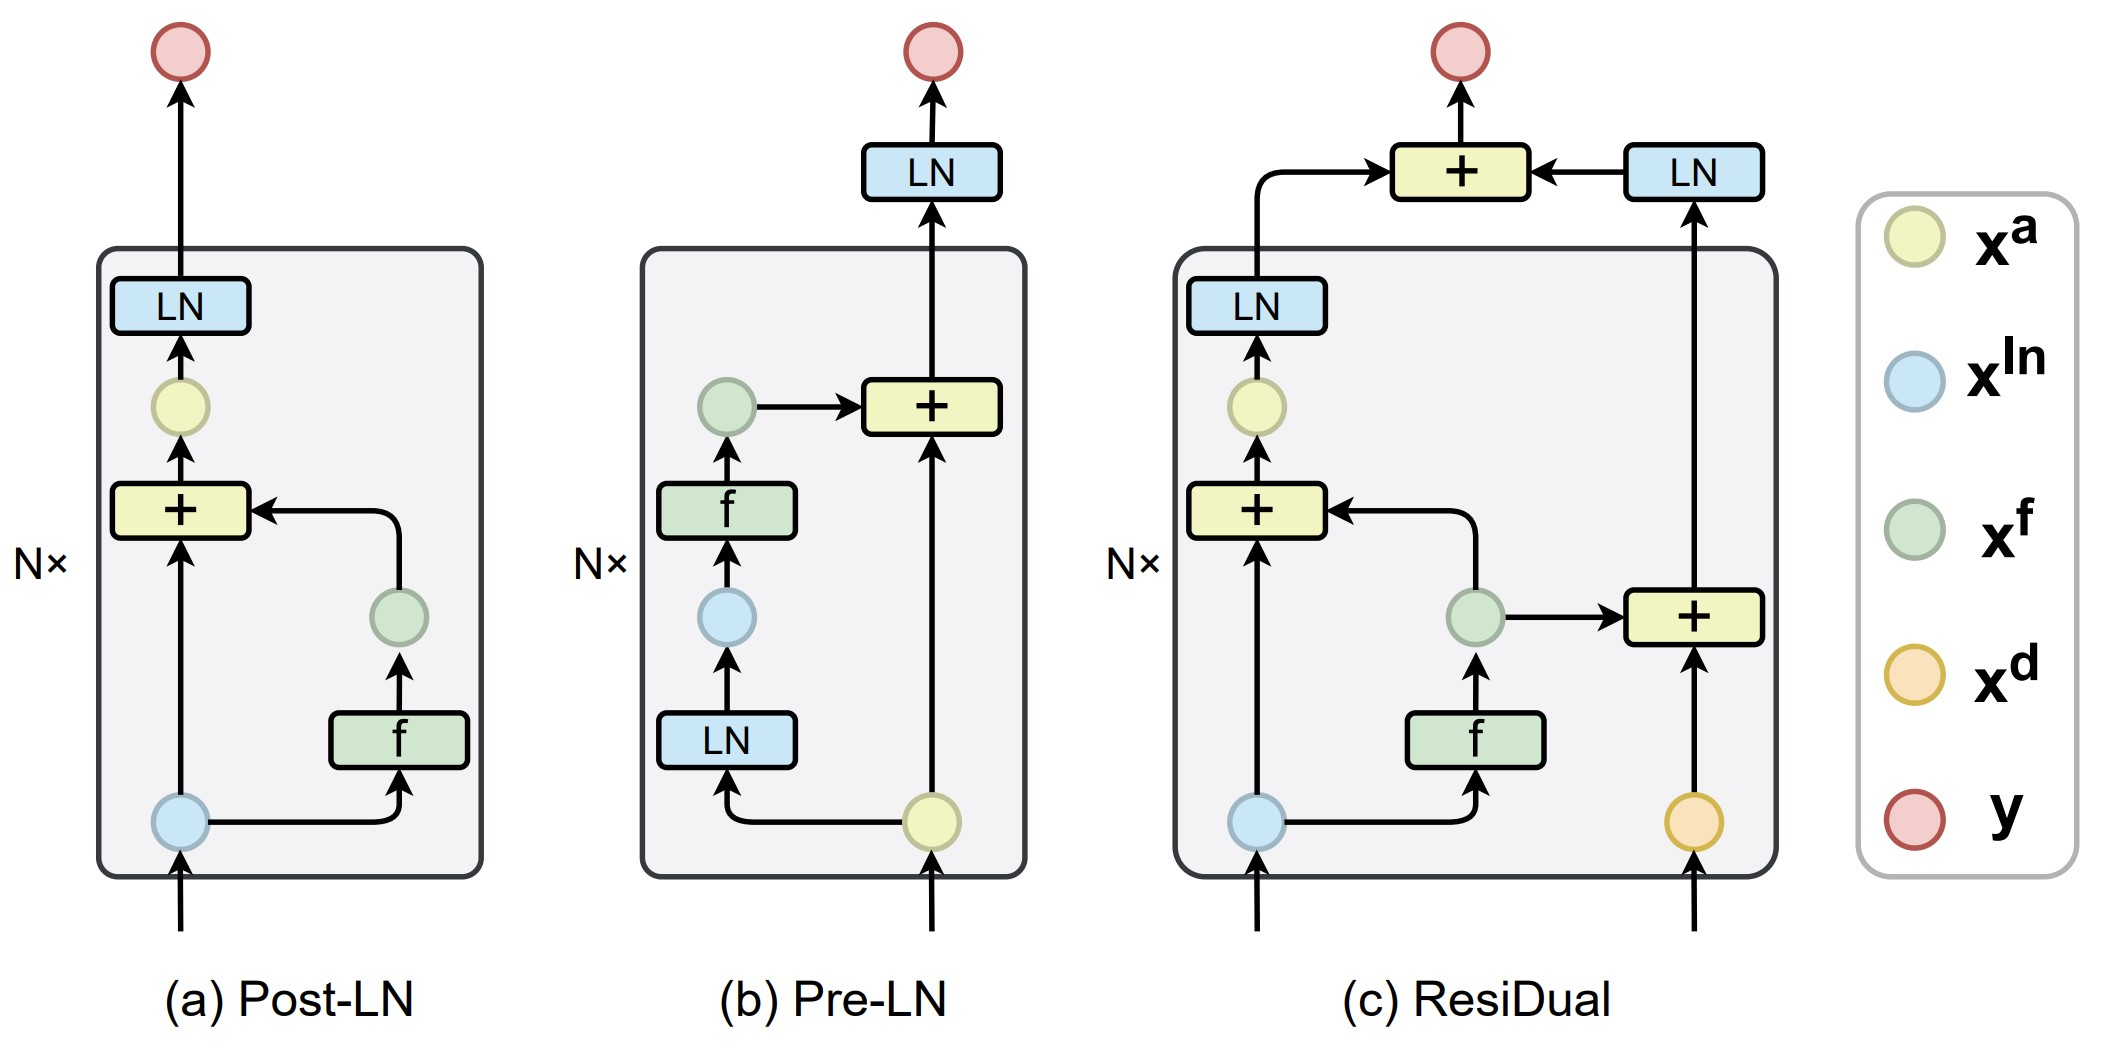
\includegraphics[width=1\linewidth]{image/residual.jpg}
    \caption{Overview of Post-LN, Pre-LN, and ResiDual. Circles with different colors represent different variables and rectangles represent different operations.}
    \label{fig:residual}
\end{figure}

The ResiDual architecture utilizes \textbf{two parallel residual branches}:

\begin{itemize}
    \item \textbf{Main Branch (Post-LN-like)}: This branch retains the structure of Post-LN, where the sub-block's output is added to its input and then normalized. This branch is crucial for \textbf{maintaining representation diversity}, which helps combat the ``representation collapse'' phenomenon often observed in Pre-LN.
    
    \item \textbf{Dual Branch (Pre-LN-like)}: A second residual path is added, allowing the signal (both forward and backward) to bypass the blocks. This branch accumulates the outputs of the sub-blocks and allows the gradient to flow directly to the deepest layers without being attenuated by normalization layers. This effectively \textbf{solves the gradient vanishing problem}.
\end{itemize}

\subsubsection*{Benefits of Adopting ResiDual:}

\begin{itemize}
    \item \textbf{Stable Training and Better Convergence}: By providing an unimpeded path for the gradient, ResiDual makes the training process significantly more stable, especially as model depth increases. This reduces the dependency on techniques like learning-rate warm-up.

    \item \textbf{Enhanced Representation Capacity}: The architecture prevents representation collapse, ensuring that deeper layers can continue to effectively learn and refine features. This allows the model to fully leverage its parameters, leading to a more powerful and robust model.
\end{itemize}